%%%%%%%%%%%%%%%%%%%%%%%%%%%%%%%%%%%%%%%%%%%%%%%%%%%%%%%%%%%%%%%%%%%%%%%%%%%%%%
%% AMS-LaTeX Paper
%%%%%%%%%%%%%%%%%%%%%%%%%%%%%%%%%%%%%%%%%%%%%%%%%%%%%%%%%%%%%%%%%%%%%%%%%%%%%%
\documentclass[12pt,leqno]{amsart}
\pdfoutput=1
\usepackage{amsmath, amssymb, amsthm}
\usepackage[svgnames]{xcolor}
\usepackage{tikz}
\usetikzlibrary{arrows,cd}
\tikzset{>=latex}
% \usepackage{mathtools}
% \usepackage[alwaysadjust]{paralist}
\usepackage[shortalphabetic]{amsrefs}
\usepackage[T1]{fontenc}
\usepackage{mathptmx}
\usepackage{microtype}
\usepackage[scaled=0.75]{beramono}
\linespread{1.06}
\usepackage[colorlinks = true,
  linkcolor  = DarkBlue,
  urlcolor   = DarkRed,
  citecolor  = DarkGreen]{hyperref}
% \hypersetup{
%   pdftitle={The simplicial complexes package for Macaulay2},
%   pdfauthor={Ben Hersey, Gregory G. Smith, and Alexandre Zotine}
% }
%% --Extras------------------------------------------------------------------
\usepackage{caption}
\usepackage{subcaption}
%% --LAYOUT-------------------------------------------------------------------
\usepackage[centering, includeheadfoot, hmargin=0.95in, tmargin=0.8in,
  bmargin=0.8in, headheight=6pt]{geometry}
%% --DISPLAY CODE------------------------------------------------------------
\usepackage{listings}
\lstset{
  basicstyle=\ttfamily,
  mathescape
}
\usepackage{stix}
%% --OTHER ENVIRONMENTS-------------------------------------------------------
\newtheorem{lemma}{Lemma}[section]
\newtheorem{theorem}[lemma]{Theorem}
\newtheorem{maintheorem}{Theorem}
\newtheorem{corollary}[lemma]{Corollary}
\newtheorem{proposition}[lemma]{Proposition}
\theoremstyle{definition}
\newtheorem{definition}[lemma]{Definition}
\newtheorem{remark}[lemma]{Remark}
\newtheorem{example}[lemma]{Example}
% \newenvironment{example}
% {\pushQED{\qed}\renewcommand{\qedsymbol}{$\diamond$}\examplex}
% {\popQED\endexamplex}
\newtheorem{question}[lemma]{Question}
\renewcommand{\theequation}{\arabic{section}.\arabic{lemma}.\arabic{equation}}
\renewcommand{\thetable}{\arabic{section}.\arabic{lemma}.\arabic{equation}}
\renewcommand{\thesubsection}{\arabic{section}}

%% --MATH---------------------------------------------------------------------
\newcommand{\colequal}{\ensuremath{:\!=}}
\newcommand{\PP}{\ensuremath{\mathbb{P}}}
%% Operators
\DeclareMathOperator{\Hom}{Hom}
\DeclareMathOperator{\Proj}{Proj}
\DeclareMathOperator{\Spec}{Spec}
\DeclareUnicodeCharacter{039A}{\Kappa}
\DeclareUnicodeCharacter{0393}{\Gamma}
\DeclareUnicodeCharacter{0394}{\Delta}
\DeclareUnicodeCharacter{22C8}{\bowtie}
\DeclareUnicodeCharacter{29D3}{\fbowtie}
\DeclareUnicodeCharacter{2119}{\mathbb{P}}

%\DeclareUnicodeCharacter{}


%%%%%%%%%%%%%%%%%%%%%%%%%%%%%%%%%%%%%%%%%%%%%%%%%%%%%%%%%%%%%%%%%%%%%%%%%%%%%%
\begin{document}

\vspace*{-4.5em}

\title[Simplicial Complexes]{Simplicial complexes in Macaulay2}

\author[B.~Hersey]{Ben Hersey}
\author[G.G.~Smith]{Gregory G.{} Smith} 
\author[A.~Zotine]{Alexandre Zotine}

\address{Department of Mathematics and Statistics, Queen's
  University, Kingston, Ontario, K7L 3N6
  {\normalfont\texttt{hersey.b@queensu.ca}},
  {\normalfont\texttt{ggsmith@mast.queensu.ca}},
  {\normalfont\texttt{18az45@queensu.ca}}.
}

\thanks{2020 \emph{Mathematics Subject Classification}. 05E45, 13F55,
  55U10\\
  %
  \indent
  \texttt{SimplicialComplexes} version 2.0
}
% \date{2021--08--20}

\begin{abstract}
  We highlight some features of the \emph{SimplicialComplexes} package in
  \emph{Macaulay2}.
\end{abstract}

\maketitle

\vspace{-0.5em}

%%%%%%%%%%%%%%%%%%%%%%%%%%%%%%%%%%%%%%%%%%%%%%%%%%%%%%%%%%%%%%%%%%%%%%%%%%%%%%
\noindent
This updated version of the \emph{SimplicialComplexes} package in
\emph{Macaulay2}~\cite{M2}, originally developed by Sorin Popescu, Gregory
G. Smith, and Mike Stillman, adds constructors for many classic examples,
implements a new data type for simplicial maps, and incorporates many
improvements to the methods and documentation.  Emphasizing combinatorial and
algebraic applications, the primary data type encodes an abstract simplicial
complex---a family of subsets that is closed under taking subsets.  These
simplicial complexes should not be conflated with their geometric realizations
formed from points, line segments, filled-in triangles, solid tetrahedra, and
their higher-dimensional analogues in some Euclidean space.  The subsets in a
simplicial complex are called its faces, the faces having cardinality~$1$ are
its vertices, and the maximal faces (ordered by inclusion) are its facets.
Following the combinatorial conventions, every nonempty simplicial complex has
the empty set as a face.

In this package, a simplicial complex is represented by its Stanley--Reisner
ideal. The vertices are identified with a subset of the variables in a
polynomial ring and each face is identified with the product of the
corresponding variables.  A nonface is any subset of the variables that does
not belong to the simplicial complex and each nonface is again identified with
a product of variables. The Stanley--Reisner ideal of a simplicial complex is
generated by monomials corresponding to its nonfaces; see Definition~5.1.2 in
\cite{BH}, Definition~1.6 in \cite{MS}, or Definition~II.1.1 in
\cite{Stanley}. Because computations in the associated polynomial ring are
typically prohibitive, this package is not intended for simplicial complexes
with a large number of vertices.

%% ---------------------------------------------------------------------------
\subsection*{\scshape\mdseries Constructors}

The basic constructor for a simplicial complex accepts two different kinds of
input.  Given a list of monomials, it returns the smallest simplicial complex
containing the corresponding faces.  Given a radical monomial ideal, it
returns the simplicial complex having the input as its Stanley--Reisner
ideal. We illustrate both methods using the `bowtie' complex appearing in
Figure~\ref{bowtie}.

\begin{figure}[t]
  \begin{subfigure}{0.3\textwidth}
    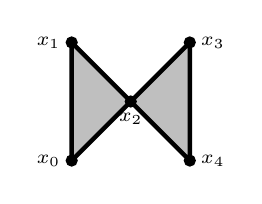
\begin{tikzpicture}
      \draw[fill=gray!50, ultra thick] (0,0) node[left]{\scriptsize $x_0$} --
      (0,1.50) node[left]{\scriptsize $x_1$} -- (0.75,0.75)
      node[below]{\scriptsize $x_2$} -- cycle;
      \draw[fill=gray!50, ultra thick] (1.50,0) node[right]{\scriptsize $x_4$} --
      (1.50,1.50) node[right]{\scriptsize $x_3$} -- (0.75,0.75) -- cycle;
      \filldraw (0,0) circle (2pt);
      \filldraw (0,1.50) circle (2pt);
      \filldraw (0.75,0.75) circle (2pt);
      \filldraw (1.50,0) circle (2pt);
      \filldraw (1.50,1.50) circle (2pt);
    \end{tikzpicture}
  \end{subfigure}
  \hspace{50pt}
  \begin{subfigure}{0.3\textwidth}
    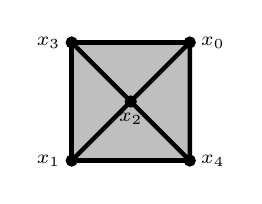
\begin{tikzpicture}
      \draw[fill=gray!50, ultra thick] (0,0) -- (1.50,0) -- (1.50,1.50) --
      (0,1.50) -- cycle;
      \draw[ultra thick] (0,0) node[left]{\scriptsize $x_1$} -- (0,1.50)
      node[left]{\scriptsize $x_3$} -- (0.75,0.75)
      node[below]{\scriptsize $x_2$} -- cycle;
      \draw[fill=gray!50, ultra thick] (1.50,0) node[right]{\scriptsize $x_4$}
      -- (1.50,1.50) node[right]{\scriptsize $x_0$} -- (0.75,0.75) -- cycle;
      \filldraw (0,0) circle (2pt);
      \filldraw (0,1.50) circle (2pt);
      \filldraw (0.75,0.75) circle (2pt);
      \filldraw (1.50,0) circle (2pt);
      \filldraw (1.50,1.50) circle (2pt);
    \end{tikzpicture}
  \end{subfigure}
  \caption{The left is the bowtie complex $⧓$ and the right its Alexander dual $⧓^*$}
  \label{bowtie}
\end{figure}

\begin{lstlisting}[xleftmargin=10pt, lineskip=-5pt, aboveskip=3.0pt, belowskip=1.5pt]
Macaulay2, version 1.18
with packages: ConwayPolynomials, Elimination, IntegralClosure, InverseSystems, 
               LLLBases, MinimalPrimes, PrimaryDecomposition, ReesAlgebra, 
               Saturation, TangentCone
\end{lstlisting}
\begin{lstlisting}[xleftmargin=10pt, aboveskip=1.5pt, belowskip=1.5pt]
i1 : needsPackage "SimplicialComplexes";
\end{lstlisting}
\begin{lstlisting}[xleftmargin=10pt, aboveskip=1.5pt, belowskip=1.5pt]
i2 : S = QQ[x_0..x_4];
\end{lstlisting}
\begin{lstlisting}[xleftmargin=10pt, aboveskip=1.5pt, belowskip=1.5pt]
i3 : $⧓$ = simplicialComplex {x_0*x_1*x_2, x_2*x_3*x_4}
\end{lstlisting}
\begin{lstlisting}[xleftmargin=10pt, aboveskip=1.5pt, belowskip=1.5pt]
o3 = simplicialComplex | x_2x_3x_4 x_0x_1x_2 |
\end{lstlisting}
\begin{lstlisting}[xleftmargin=10pt, aboveskip=1.5pt, belowskip=1.5pt]
o3 : SimplicialComplex
\end{lstlisting}
\begin{lstlisting}[xleftmargin=10pt, aboveskip=1.5pt, belowskip=1.5pt]
i4 : I = monomialIdeal $⧓$
\end{lstlisting}
\begin{lstlisting}[xleftmargin=10pt, lineskip=-10pt, aboveskip=4pt, belowskip=1.5pt]
o4 = monomialIdeal (x x , x x , x x , x x )
                     0 3   1 3   0 4   1 4
\end{lstlisting}
\begin{lstlisting}[xleftmargin=10pt, aboveskip=1.5pt, belowskip=1.5pt]
o4 : MonomialIdeal of S
\end{lstlisting}
\begin{lstlisting}[xleftmargin=10pt, aboveskip=1.5pt, belowskip=1.5pt]
i5 : $⧓$' = simplicialComplex I
\end{lstlisting}
\begin{lstlisting}[xleftmargin=10pt, aboveskip=1.5pt, belowskip=1.5pt]
o5 = simplicialComplex | x_2x_3x_4 x_0x_1x_2 |
\end{lstlisting}
\begin{lstlisting}[xleftmargin=10pt, aboveskip=1.5pt, belowskip=1.5pt]
o5 : SimplicialComplex
\end{lstlisting}
\begin{lstlisting}[xleftmargin=10pt, aboveskip=1.5pt, belowskip=3.0pt]
i6 : assert($⧓$ === $⧓$')
\end{lstlisting}

The package also has convenience constructors for some archetypal simplicial
complexes. For example, we recognize triangulations of the real projective
plane and the Klein bottle from their reduced homology groups; see
Theorems~6.3--6.4 in \cite{Munkres}.
\begin{lstlisting}[xleftmargin=10pt, lineskip=-5pt, aboveskip=3.0pt, belowskip=1.5pt]
i7 : $ℙ$ = realProjectiveSpaceComplex(2, R = ZZ[a..h])
\end{lstlisting}
\begin{lstlisting}[xleftmargin=10pt, aboveskip=1.5pt, belowskip=1.5pt]
o7 = simplicialComplex | bef aef cdf adf bcf cde bde ace abd abc |
\end{lstlisting}
\begin{lstlisting}[xleftmargin=10pt, aboveskip=1.5pt, belowskip=1.5pt]
o7 : SimplicialComplex
\end{lstlisting}
\begin{lstlisting}[xleftmargin=10pt, aboveskip=1.5pt, belowskip=1.5pt]
i8 : for j from 0 to 2 list prune HH_j $ℙ$
\end{lstlisting}
\begin{lstlisting}[xleftmargin=10pt, aboveskip=1.5pt, belowskip=1.5pt]
o8 = {0, cokernel | 2 |, 0}
\end{lstlisting}
\begin{lstlisting}[xleftmargin=10pt, aboveskip=1.5pt, belowskip=1.5pt]
o8 : List
\end{lstlisting}
\begin{lstlisting}[xleftmargin=10pt, aboveskip=1.5pt, belowskip=1.5pt]
i9 : for j from 0 to 2 list prune HH_j kleinBottleComplex R
\end{lstlisting}
\begin{lstlisting}[xleftmargin=10pt, lineskip=-10pt, aboveskip=4pt, belowskip=1.5pt]
o9 = {0, cokernel | 2 |, 0}
                  | 0 |
\end{lstlisting}
\begin{lstlisting}[xleftmargin=10pt, aboveskip=-5pt, belowskip=3.0pt]
o9 : List
\end{lstlisting}
More comprehensively, Frank H.~Lutz enumerates simplicial complexes having a
small number of vertices; see \cite{LutzM}.  Using this list, the package
creates a database of $43\,138$ simplicial $2$\nobreakdash-manifolds having at
most $10$ vertices and $1\,343$ simplicial $3$-manifolds having at most $9$
vertices.  We demonstrate this feature by exhibiting the distribution of
$f\!$-vectors among the $3$-manifolds having $9$ vertices.  For all nonnegative
integers $j$, the $j$-th entry in the $f\!$-vector is the number of faces having
$j$ vertices.
\begin{lstlisting}[xleftmargin=10pt, lineskip=-5pt, aboveskip=3.0pt, belowskip=1.5pt]
i10 : tally for j from 0 to 1296 list 
          fVector smallManifold(3, 9, j, ZZ[vars(1..9)])
\end{lstlisting}
\begin{lstlisting}[xleftmargin=10pt, lineskip=-5pt, aboveskip=4pt, belowskip=1.5pt]
o10 = Tally{{1, 9, 26, 34, 17} => 7  }
            {1, 9, 27, 36, 18} => 23
            {1, 9, 28, 38, 19} => 45
            {1, 9, 29, 40, 20} => 84
            {1, 9, 30, 42, 21} => 128
            {1, 9, 31, 44, 22} => 175
            {1, 9, 32, 46, 23} => 223
            {1, 9, 33, 48, 24} => 231
            {1, 9, 34, 50, 25} => 209
            {1, 9, 35, 52, 26} => 121
            {1, 9, 36, 54, 27} => 51
\end{lstlisting}
\begin{lstlisting}[xleftmargin=10pt, aboveskip=-5pt, belowskip=3.0pt]
o10 : Tally
\end{lstlisting}
Exploiting the same loop, we construct the simplicial maps from a minimal
triangulation of a torus to the induced subcomplex on the first $7$ vertices
for each of these $3$-manifolds.
\begin{lstlisting}[xleftmargin=10pt, aboveskip=3.0pt, belowskip=1.5pt]
i11 : T = smallManifold(2, 7, 1, R = ZZ[a..i])
\end{lstlisting}
\begin{lstlisting}[xleftmargin=10pt, aboveskip=1.5pt, belowskip=1.5pt]
o11 = simplicialComplex | dfg afg deg aeg adf cde ace bcd abd abc |
\end{lstlisting}
\begin{lstlisting}[xleftmargin=10pt, aboveskip=1.5pt, belowskip=1.5pt]
o11 : SimplicialComplex
\end{lstlisting}
\begin{lstlisting}[xleftmargin=10pt, aboveskip=1.5pt, belowskip=1.5pt]
i12 : gens monomialIdeal T
\end{lstlisting}
\begin{lstlisting}[xleftmargin=10pt, aboveskip=1.5pt, belowskip=1.5pt]
o12 = | acd be ade bf cf ef bg cg adg h i |
\end{lstlisting}
\begin{lstlisting}[xleftmargin=10pt, lineskip=-10pt, aboveskip=4pt, belowskip=1.5pt]
              1       11
o12 : Matrix R  <--- R
\end{lstlisting}
\begin{lstlisting}[xleftmargin=10pt, aboveskip=1.5pt, belowskip=1.5pt]
i13 : for j from 0 to 2 list prune HH_j T
\end{lstlisting}
\begin{lstlisting}[xleftmargin=10pt, lineskip=-10pt, aboveskip=4pt, belowskip=1.5pt]
               1
o13 = {0, 0, ZZ }
\end{lstlisting}
\begin{lstlisting}[xleftmargin=10pt, aboveskip=1.5pt, belowskip=1.5pt]
o13 : List
\end{lstlisting}
\begin{lstlisting}[xleftmargin=10pt, lineskip=-10pt, aboveskip=4pt, belowskip=1.5pt]
i14 : mapList = for j from 0 to 1296 list (
          phi := map(smallManifold(3, 9, j, S), T, gens R);
          if not isWellDefined phi then continue else phi);
\end{lstlisting}
\begin{lstlisting}[xleftmargin=10pt, aboveskip=1.5pt, belowskip=1.5pt]
i15 : # mapList
\end{lstlisting}
\begin{lstlisting}[xleftmargin=10pt, aboveskip=1.5pt, belowskip=1.5pt]
o15 = 319
\end{lstlisting}
\begin{lstlisting}[xleftmargin=10pt, aboveskip=1.5pt, belowskip=-5.0pt]
i16 : assert all(mapList, phi -> isInjective phi)
\end{lstlisting}


%% ---------------------------------------------------------------------------
\subsection*{\scshape\mdseries Combinatorial Topology}

We showcase some of the key operations on simplicial complex using the bowtie
complex.  Viewing a simplicial complex as lying in a standard simplex yields a
duality theory. For any simplicial complex $\Delta$ whose vertices belong to a
set $V$, the Alexander dual is the simplicial complex
$\Delta^* \colequal \{ F \subseteq V \mathrel{|} V \setminus F \in \Delta \}$.
Since each simplicial complex in this package has an underlying polynomial
ring, the variables in this ring form the canonical superset of vertices.
\begin{lstlisting}[xleftmargin=10pt, aboveskip=3.0pt, belowskip=1.5pt]
i17 : dual $⧓$
\end{lstlisting}
\begin{lstlisting}[xleftmargin=10pt, aboveskip=1.5pt, belowskip=1.5pt]
o17 = simplicialComplex | x_1x_2x_4 x_0x_2x_4 x_1x_2x_3 x_0x_2x_3 |
\end{lstlisting}
\begin{lstlisting}[xleftmargin=10pt, aboveskip=1.5pt, belowskip=1.5pt]
o17 : SimplicialComplex
\end{lstlisting}
\begin{lstlisting}[xleftmargin=10pt, aboveskip=1.5pt, belowskip=1.5pt]
i18 : assert(dual dual $⧓$ === $⧓$)
\end{lstlisting}
\begin{lstlisting}[xleftmargin=10pt, aboveskip=1.5pt, belowskip=3pt]
i19 : assert(dual monomialIdeal $⧓$ === monomialIdeal dual $⧓$)
\end{lstlisting}
Algebraically, Alexander duality switches the roles of minimal generators and
irreducible components in the Stanley--Reisner ideal.
\begin{lstlisting}[xleftmargin=10pt, aboveskip=3pt, belowskip=1.5pt]
i20 : monomialIdeal dual $⧓$
\end{lstlisting}
\begin{lstlisting}[xleftmargin=10pt, lineskip=-10pt, aboveskip=4pt, belowskip=1pt]
o20 = monomialIdeal (x x , x x )
                      0 1   3 4
\end{lstlisting}
\begin{lstlisting}[xleftmargin=10pt, aboveskip=1.5pt, belowskip=1.5pt]
o20 : MonomialIdeal of S
\end{lstlisting}
\begin{lstlisting}[xleftmargin=10pt, aboveskip=1.5pt, belowskip=1.5pt]
i21 : irreducibleDecomposition monomialIdeal $⧓$
\end{lstlisting}
\begin{lstlisting}[xleftmargin=10pt, lineskip=-10pt, aboveskip=4pt, belowskip=1pt]
o21 = {monomialIdeal (x , x ), monomialIdeal (x , x )}
                       0   1                   3   4
\end{lstlisting}
\begin{lstlisting}[xleftmargin=10pt, aboveskip=1pt, belowskip=3pt]
o21 : List
\end{lstlisting}
The topological form of Alexander duality gives an isomorphism
between the reduced homology of a simplicial complex and reduced cohomology of
its dual; see Theorem~5.6 in \cite{MS}.
\begin{lstlisting}[xleftmargin=10pt, aboveskip=3pt, belowskip=1.5pt]
i22 : n = numgens ring $⧓$;
\end{lstlisting}
\begin{lstlisting}[xleftmargin=10pt, aboveskip=1pt, belowskip=3pt]
i23 : assert all(-1..n-1, j -> prune HH^(n-j-3) dual $⧓$ == prune HH_j $⧓$)
\end{lstlisting}

A simplicial complex $\Delta$ is Cohen--Macaulay if the associated quotient
ring $S/I$, where $I$ is the Stanley--Reisner ideal of $\Delta$ in the
polynomial ring $S$, is Cohen--Macaulay.  To characterize this attribute
topologically, we introduce a family of subcomplexes.  For any face $F$ in
$\Delta$, the link is the subcomplex
$\operatorname{link}_\Delta(F) \colequal \{ G \in \Delta \mathrel{|}
\text{$F \cup G \in \Delta$ and $F \cap G = \varnothing$} \}$.  The link of
the vertex $x_2$ in $⧓$ has two disjoint facets.
\begin{lstlisting}[xleftmargin=10pt, aboveskip=3.0pt, belowskip=1.5pt]
i24 : L = link($⧓$, x_2)
\end{lstlisting}
\begin{lstlisting}[xleftmargin=10pt, aboveskip=1.5pt, belowskip=1.5pt]
o24 = simplicialComplex | x_3x_4 x_0x_1 |
\end{lstlisting}
\begin{lstlisting}[xleftmargin=10pt, aboveskip=1.5pt, belowskip=1.5pt]
o24 : SimplicialComplex
\end{lstlisting}
\begin{lstlisting}[xleftmargin=10pt, aboveskip=1.5pt, belowskip=1.5pt]
i25 : prune HH_0 L
\end{lstlisting}
\begin{lstlisting}[xleftmargin=10pt, lineskip=-10pt, aboveskip=4pt, belowskip=1pt]
        1
o25 = QQ
\end{lstlisting}
\begin{lstlisting}[xleftmargin=10pt, aboveskip=1.5pt, belowskip=3.0pt]
o25 : QQ-module, free
\end{lstlisting}
The dimension of a simplicial complex is one less than the maximal cardinality
of its faces.
\begin{lstlisting}[xleftmargin=10pt, aboveskip=3.0pt, belowskip=1.5pt]
i26 : dim L
\end{lstlisting}
\begin{lstlisting}[xleftmargin=10pt, aboveskip=1.5pt, belowskip=3.0pt]
o26 = 1
\end{lstlisting}
As discovered by Gerald Reisner, the simplicial complex $\Delta$ is
Cohen--Macaulay if and only if, for all faces $F$ in $\Delta$ and all integers
$j$ less than the dimension of $\operatorname{link}_\Delta(F)$, the $j$-th
reduced homology group of $\operatorname{link}_\Delta(F)$ vanishes; see
Corollary~5.3.9 in \cite{BH}, Theorem~5.53 in \cite{MS}, or Corollary~II.4.2
in \cite{Stanley}.  Using this criterion, the $0$-th reduced homology
certifies that $⧓$ is not Cohen--Macaulay.
\begin{lstlisting}[xleftmargin=10pt, aboveskip=3.0pt, belowskip=1.5pt]
i27 : assert(HH_0 L != 0)
\end{lstlisting}
\begin{lstlisting}[xleftmargin=10pt, aboveskip=1.5pt, belowskip=3.0pt]
i28 : assert(dim(S^1/monomialIdeal $⧓$) =!= n - pdim(S^1/monomialIdeal $⧓$))
\end{lstlisting}
However, the $1$-skeleton of $⧓$ is Cohen--Macaulay.
\begin{lstlisting}[xleftmargin=10pt, aboveskip=3.0pt, belowskip=1.5pt]
i29 : $⋈$ = skeleton(1, $⧓$)
\end{lstlisting}
\begin{lstlisting}[xleftmargin=10pt, aboveskip=1.5pt, belowskip=1.5pt]
o29 = simplicialComplex | x_3x_4 x_2x_4 x_2x_3 x_1x_2 x_0x_2 x_0x_1 |
\end{lstlisting}
\begin{lstlisting}[xleftmargin=10pt, aboveskip=1.5pt, belowskip=1.5pt]
o29 : SimplicialComplex
\end{lstlisting}
\begin{lstlisting}[xleftmargin=10pt, aboveskip=1.5pt, belowskip=1.5pt]
i30 : faceList = rsort flatten values faces $⋈$
\end{lstlisting}
\begin{lstlisting}[xleftmargin=10pt, lineskip=-10pt, aboveskip=4pt, belowskip=1pt]
o30 = {x x , x x , x x , x x , x x , x x , x , x , x , x , x , 1}
        0 1   0 2   1 2   2 3   2 4   3 4   0   1   2   3   4
\end{lstlisting}
\begin{lstlisting}[xleftmargin=10pt, aboveskip=1.5pt, belowskip=1.5pt]
o30 : List
\end{lstlisting}
\begin{lstlisting}[xleftmargin=10pt, aboveskip=1.5pt, belowskip=1.5pt]
i31 : assert all(faceList, F -> (L := link($⋈$, F); all(dim L, j -> HH_j L == 0)))
\end{lstlisting}
\begin{lstlisting}[xleftmargin=10pt, aboveskip=1.5pt, belowskip=3.0pt]
i32 : assert(dim(S^1/monomialIdeal $⋈$) === n - pdim(S^1/monomialIdeal $⋈$))
\end{lstlisting}

Alternatively, we verify that bowtie complex $⧓$ is not Cohen--Macaulay by
showing that its $h$-vector has a negative entry; see Theorem~5.1.10 in
\cite{BH} or Corollary~II.2.5 in \cite{Stanley}.  By definition, the
$h$-vector of a simplicial complex $\Delta$ is a binomial transform of its
$f\!$-vector: for all $0 \leqslant j \leqslant d \colequal \dim \Delta$, we have
$h_j = \sum_{k=0}^{j} (-1)^{j-1}
\smash{\tbinom{d+1-k}{\raisebox{3pt}{$\scriptstyle j-k$}}} f_{k-1}$.  The
$h$-vector encodes the numerator of the Hilbert series for $S/I$.

\begin{lstlisting}[xleftmargin=10pt, aboveskip=3.0pt, belowskip=1.5pt]
i33 : d = dim $⧓$
\end{lstlisting}
\begin{lstlisting}[xleftmargin=10pt, aboveskip=1.5pt, belowskip=1.5pt]
o33 = 2
\end{lstlisting}
\begin{lstlisting}[xleftmargin=10pt, aboveskip=1.5pt, belowskip=1.5pt]
i34 : faces $⧓$
\end{lstlisting}
\begin{lstlisting}[xleftmargin=10pt, lineskip=-10pt, aboveskip=4pt, belowskip=1pt]
o34 = HashTable{-1 => {1}                                }
                0 => {x , x , x , x , x }
                       0   1   2   3   4
                1 => {x x , x x , x x , x x , x x , x x }
                       0 1   0 2   1 2   2 3   2 4   3 4
                2 => {x x x , x x x }
                       0 1 2   2 3 4
\end{lstlisting}
\begin{lstlisting}[xleftmargin=10pt, aboveskip=1.5pt, belowskip=1.5pt]
o34 : HashTable
\end{lstlisting}
\begin{lstlisting}[xleftmargin=10pt, aboveskip=1.5pt, belowskip=1.5pt]
i35 : fVec = fVector $⧓$
\end{lstlisting}
\begin{lstlisting}[xleftmargin=10pt, aboveskip=1.5pt, belowskip=1.5pt]
o35 = {1, 5, 6, 2}
\end{lstlisting}
\begin{lstlisting}[xleftmargin=10pt, aboveskip=1.5pt, belowskip=1.5pt]
o35 : List
\end{lstlisting}
\begin{lstlisting}[xleftmargin=10pt, lineskip=-10pt, aboveskip=4pt, belowskip=1pt]
i36 : hVec = for j from 0 to d list 
          sum(j+1, k -> (-1)^(j-k) * binomial(d+1-k, j-k) * fVec#k)
\end{lstlisting}
\begin{lstlisting}[xleftmargin=10pt, aboveskip=1.5pt, belowskip=1.5pt]
o36 = {1, 2, -1}
\end{lstlisting}
\begin{lstlisting}[xleftmargin=10pt, aboveskip=1.5pt, belowskip=1.5pt]
o36 : List
\end{lstlisting}
\begin{lstlisting}[xleftmargin=10pt, aboveskip=1.5pt, belowskip=1.5pt]
i37 : hilbertSeries(S^1/monomialIdeal $⧓$, Reduce => true)
\end{lstlisting}
\begin{lstlisting}[xleftmargin=10pt, lineskip=-10pt, aboveskip=4pt, belowskip=1pt]
                2
      1 + 2T - T
o37 = -----------
               3
        (1 - T)
\end{lstlisting}
\begin{lstlisting}[xleftmargin=10pt, aboveskip=1.5pt, belowskip=-5.0pt]
o37 : Expression of class Divide
\end{lstlisting}


%% ---------------------------------------------------------------------------
\subsection*{\scshape\mdseries Resolutions of Monomial Ideals}

In this section, we will overview
some chain complex constructions arising from simplicial complexes. We give an
example of ideal homogenization and resolutions supported on a simplicial
complex, and we provide examples of Taylor, Lyubeznik, and Buchberger
resolutions; as well as Scarf complexes.

Let $\Delta$ be a simplicial complex with $q$ vertices and let
$\widetilde C(\Delta;k)$ be the augmented chain complex of $\Delta$ with
incidence function $\varepsilon$. We will let $S = k[x_0,\dotsc,x_n]$ be a
polynomial ring over the commutative ring $k$, which is typically a field. We
assume that the ring $S$ has the fine $\mathbb N^{n+1}$ grading.

For a monomial ideal $I \subset S$, minimally generated by
$m_1,m_2,\dotsc,m_q$, a \textbf{labelling} of $\Delta$ by $I$ is a bijection
which assigns a minimal generator of $I$ to each vertex of $\Delta$. Without
loss of generality, we will assume this assignment is $v_i \longmapsto m_i$
for $i = 1,2,\dotsc,q$. For each face $F \in \Delta$ we can construct the
monomial $m_F = \mathrm{lcm}(m_i \ | \ i \in F )$. The
$I$-\textbf{homogenization} of $\widetilde{C} (\Delta;k)$ is the chain complex
$(\mathbf G, d)$ such that
%
\begin{displaymath}
  G_0 = S \ \text{ and } \ G_i = \bigoplus_{\dim(F) = i-1}S(m_F).
\end{displaymath}
%
We will use $\{f_F \ | \ F \in \Delta \}$ to denote the canonical basis of $G$ and we define the differential of $\mathbf G$ using
%
\begin{displaymath}
  d(f_F) \hspace{4pt} = \hspace{-8pt} \sum_{\dim(F) = i-1} \frac{m_F}{m_{F'}} \cdot \varepsilon(F,F') f_{F'}.
\end{displaymath}
%
We say that $I$ has a \textbf{resolution supported on} $\Delta$ if the
$I$-homogenization of $\widetilde C(\Delta; k)$ is a free resolution for some
labelling of the vertices of $\Delta$. For further details on
$I$-homogenization, we refer the reader to any one of \cites{MS, Peeva}.


Let $S = \mathbb Q[x_0,x_1,x_2,x_3]$, let
$I = (x_0x_1,x_0x_2,x_0x_3,x_1x_2x_3)$, and let $\Gamma$ be the simplicial
complex with facets $\{ v_1,v_2,v_3 \}$ and $\{ v_2, v_4 \}$.  If we use the
labelling $v_1 \longmapsto x_0x_1$, $v_2 \longmapsto x_0x_2$,
$v_3 \longmapsto x_0x_3$, and $v_4 \longmapsto x_1x_2x_3$, we get the labelled
simplicial complex shown in Figure \ref{Figure: Example of a labelled
  simplicial complex}.

\begin{figure}[h]\centering
  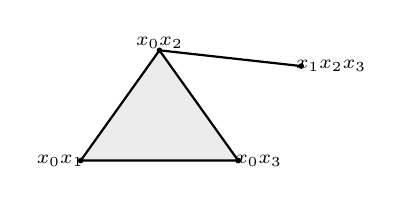
\begin{tikzpicture}[scale=.2]
    \filldraw[gray!15] (0,0) -- (10,0) -- (5,7) -- cycle;
    \draw[thick] (0,0) -- (10,0) -- (5,7) -- cycle;
    \draw[thick] (5,7) -- (14,6);
    \filldraw (0,0) circle (4pt);
    \filldraw (10,0) circle (4pt);
    \filldraw (5,7) circle (4pt);
    \filldraw (14,6) circle (4pt);
    \draw node at (-1.3,0){\scriptsize $x_0x_1$};
    \draw node at (11.3,0){\scriptsize $x_0x_3$};
    \draw node at (5,7.5){\scriptsize $x_0x_2$};
    \draw node at (15.9,6){\scriptsize $x_1x_2x_3$};
    % \draw[blue] node at (5,-.7){\scalebox{.8}{$x_1x_3x_4$}};
    % \draw[blue] node at (0.6,3.5){\scalebox{.8}{$x_1x_2x_4$}};
    % \draw[blue] node at (9.3,3.5){\scalebox{.8}{$x_2x_3x_4$}};
    % \draw[blue] node at (10,7){\scalebox{.8}{$x_1x_2x_4$}};
    % \draw[blue] node at (5,2.5){\scalebox{.8}{$x_1x_2x_3x_4$}};
  \end{tikzpicture}
  \caption{The homogenization of $\Gamma$}
  \label{Figure: Example of a labelled simplicial complex}
\end{figure}

We can use \texttt{Macaulay2} to compute both
$\widetilde C(\Delta; \mathbb Q)$ and the $I$-homogenization of $\Delta$
relative to this labelling, which is the minimal free resolution of $S/I$.
%
\begin{lstlisting}[basicstyle={\ttfamily \scriptsize}, xleftmargin=-23pt]
    i9 : R = ZZ/101[y_0..y_13];
    i10 : S = QQ[x_0..x_3];
    i11 : $Δ$ = simplicialComplex{R_0*R_1*R_2, R_2*R_3};
    i12 : I = ideal(x_0*x_1,x_0*x_2,x_0*x_3,x_1*x_2*x_3);
    o12 : Ideal of S
    i13 : C = chainComplex $Δ$
            ZZ 1       ZZ 4       ZZ 4       ZZ 1
    o13 = (---)  <-- (---)  <-- (---)  <-- (---)
           101        101        101        101
          -1         0          1          2
    o13 : ChainComplex
    i24 : G = chainComplex($Δ$, Labels => {x_0*x_1,x_0*x_2,x_0*x_3,x_1*x_2*x_3});
    i25 : G.dd
               1                                          4
    o25 = 0 : S  <-------------------------------------- S  : 1
                    | x_0x_1 x_0x_2 x_0x_3 x_1x_2x_3 |
               4                                      4
          1 : S  <---------------------------------- S  : 2
                    {2} | -x_2 -x_3 0    0       |
                    {2} | x_1  0    -x_3 0       |
                    {2} | 0    x_1  x_2  -x_1x_2 |
                    {3} | 0    0    0    x_0     |
               4                    1
          2 : S  <---------------- S  : 3
                    {3} | x_3  |
                    {3} | -x_2 |
                    {3} | x_1  |
                    {4} | 0    |
    o25 : ChainComplexMap
    i15 : (res (S^1/I)) == G
    o15 = true
\end{lstlisting}
%
The $I$-homogenization of $\Delta$ is dependent on how you label the vertices,
and that is reflected by the ordering of the monomials in the \texttt{Labels}
argument. Indeed, if we swap the labels of $v_1$ and $v_4$, then the
$I$-homogenization is no longer a resolution of $S/I$.
%
\begin{lstlisting}[basicstyle={\ttfamily \scriptsize}, xleftmargin=-23pt]
    i22 : G' = chainComplex($Δ$, Labels => {x_1*x_2*x_3,x_0*x_2,x_0*x_3,x_0*x_1});
    i23 : prune homology G'
    o23 = 0 : cokernel | x_0x_3 x_0x_2 x_0x_1 x_1x_2x_3 |
          1 : cokernel {3} | x_3 |                       
          2 : 0                                          
          3 : 0                                          
    o23 : GradedModule
\end{lstlisting}

Given a monomial ideal $I$, there are several algorithms that will produce a
simplicial complex $\Delta$ and a labelling of $\Delta$ by the minimal
generators of $I$ such that the $I$-homogenization of
$\widetilde C(\Delta; k)$ is a free resolution of $S/I$, though often
non-minimally. Examples of such constructions are the Taylor resolution,
Lyubeznik resolution, and the Buchberger resolution, all of which are
implemented in \texttt{SimplicialComplexes}. We have also implemented a
constructor for the Scarf complex, which is a complex that is not always a
free resolution of $S/I$, but when it is a free resolution it is minimal. We
will not describe these constructions here, but a concise description of the
Taylor resolution, Lyubeznik resolution, and Scarf complex is given in
\cite{Mermin}, and a description of the Buchberger resolution is given in
\cite{OW}.

Consider the monomial ideal
$I = (x_1x_3, x_2^2, x_0x_2, x_1^2, x_0^2) \subset \mathbb
C[x_0,\dotsc,x_3]$. The Taylor resolution of $I$ can be realized as an
$I$-homogenization of the $4$-simplex.
%  
\begin{lstlisting}[basicstyle={\ttfamily \scriptsize}, xleftmargin=-23pt]
    i2 : R = QQ[a,b,c,d,e];
    i3 : S = QQ[x_0..x_3];
    i4 : I = monomialIdeal(x_1*x_3, x_2^2,  x_0*x_2, x_1^2, x_0^2);
    o4 : MonomialIdeal of S
    i5 : T = taylorResolution J
          1      5      10      10      5      1
    o5 = S  <-- S  <-- S   <-- S   <-- S  <-- S
         0      1      2       3       4      5
    o5 : ChainComplex
    i6 : T == chainComplex(simplexComplex(4,R),Labels => first entries mingens I)
    o6 = true
\end{lstlisting}
  %
  The Buchberger simplicial complex is a subcomplex of the $4$-simplex, and the Buchberger resolution is an $I$-homogenization of the Buchberger simplicial complex. For this example, the Buchberger resolution is the minimal free resolution of $S/I$, but this is not always the case.
  %
\begin{lstlisting}[basicstyle={\ttfamily \scriptsize}, xleftmargin=-23pt]
    i7 : buchbergerSimplicialComplex(J,R)
    o7 = simplicialComplex | acde abcd |
    o7 : SimplicialComplex
    i8 : B = buchbergerResolution J
          1      5      9      7      2
    o8 = S  <-- S  <-- S  <-- S  <-- S
         0      1      2      3      4
    o8 : ChainComplex
    i10 : betti B === betti(res J)
    o10 = true
\end{lstlisting}
  %
Lyubeznik simplicial complexes and resolutions are constructed relative to a total order on the minimal generators of $I$. Every ordering will produce a resolution, but these resolutions need not be isomorphic. When no ordering is given, the methods \texttt{lyubeznikSimplicialComplex} and \texttt{lyubeznikResolution} will order the generators relative to the monomial order on $S$ which, in Macaulay2, is graded revlex by default. The option \texttt{MonomialOrder} reorders the minimal generators of $I$ relative to the monomial ordering on $S$. For example, \texttt{MonomialOrder => \{2,1,0,3,4\}} refers to the total ordering $x_0x_2 <  x_2^2 < x_1x_3 < x_1^2 < x_0^2$ on the minimal generators of $I$. We see that by changing the ordering we can both produce the worst case (Taylor resolution) and best case (minimal free resolution).
  %
\begin{lstlisting}[basicstyle={\ttfamily \scriptsize}, xleftmargin=-23pt]
    i11 : lyubeznikSimplicialComplex(J,R)
    o11 = simplicialComplex | abcde |
    o11 : SimplicialComplex
    i12 : lyubeznikResolution(J) == taylorResolution(J)
    o12 = true
    i13 : lyubeznikSimplicialComplex(J, R, MonomialOrder => {2,1,0,3,4})
    o13 = simplicialComplex | acde abcd |
    o13 : SimplicialComplex
    i14 : L = lyubeznikResolution(J,MonomialOrder => {2,1,0,3,4})
           1      5      9      7      2
    o14 = S  <-- S  <-- S  <-- S  <-- S
          0      1      2      3      4
    o14 : ChainComplex
\end{lstlisting}
  %
The Scarf simplicial complex of $I$ starts with the labelled $4$-simplex and removes any faces $F,F'$ such that $m_F = m_{F'}$. The $I$-homogenization of the Scarf simplicial complex is the Scarf chain complex. It is often the case that the Scarf chain complex is not a free resolution of $S/I$, but when it is a resolution, it is minimal, see \cite[Lemma 3.1]{BPS}.
  %
\begin{lstlisting}[basicstyle={\ttfamily \scriptsize}, xleftmargin=-23pt]
    i16 : scarfSimplicialComplex(J,R)
    o16 = simplicialComplex | acde abcd |
    o16 : SimplicialComplex
    i17 : scarfChainComplex J == buchbergerResolution J
    o17 = true
\end{lstlisting}



%% ---------------------------------------------------------------------------
\subsection*{\scshape\mdseries Acknowledgements}
All three authors were partially supported by the Natural Sciences and
Engineering Research Council of Canada (NSERC).


%% ---------------------------------------------------------------------------

\begin{bibdiv}
  \begin{biblist}%[\normalsize]

    \bib{MFRG}{article}{
      label={\`AFG},
      author={\`Alvarez Montaner, Josep},
      author={Fern\'{a}ndez-Ramos, Oscar},
      author={Gimenez, Philippe},
      title={Pruned cellular free resolutions of monomial ideals},
      journal={J. Algebra},
      volume={541},
      date={2020},
      pages={126--145},
      % issn={0021-8693},
      % review={\MR{4014733}},
      % doi={10.1016/j.jalgebra.2019.09.013},
    }    
    
    \bib{BH}{book}{
      author={Bruns, Winfried},
      author={Herzog, J\"{u}rgen},
      title={\href{https://doi.org/10.1017/CBO9780511608681}%
        {Cohen-Macaulay rings}},
      series={Cambridge Studies in Advanced Mathematics},
      volume={39},
      publisher={Cambridge University Press, Cambridge},
      date={1993},
      pages={xii+403},
      % isbn={0-521-41068-1},
      % review={\MR{1251956}},
      % doi={10.1017/CBO9780511608681},
    }
    
    \bib{LutzM}{webpage}{
      author={Lutz, Frank~H.},
      title={The Manifold Page},
      url={http://page.math.tu-berlin.de/~lutz/stellar/},
      date={2017},
    }

    \bib{M2}{misc}{
      label={M2},
      author={Grayson, Daniel~R.},
      author={Stillman, Michael~E.},
      title={Macaulay2, a software system for research
        in algebraic geometry},
      publisher={available at \url{http://www.math.uiuc.edu/Macaulay2/}},
    }

    \bib{Mermin}{article}{
      label={Me},      
      author={Mermin, Jeff},
      title={Three simplicial resolutions},
      conference={
        title={Progress in commutative algebra 1},
      },
      book={
        publisher={de Gruyter, Berlin},
      },
      date={2012},
      pages={127--141},
      % review={\MR{2932583}},
    }    

    \bib{MS}{book}{
      author={Miller, Ezra},
      author={Sturmfels, Bernd},
      title={Combinatorial Commutative Algebra},
      series={Graduate Texts in Mathematics},
      volume={227},
      publisher={Springer-Verlag New York},
      date={2005},
      pages={xiv+420}
      % isbn={9780387237077},
    }    

    \bib{Munkres}{book}{
      label={Mu},
      author={Munkres, James R.},
      title={Elements of algebraic topology},
      publisher={Addison-Wesley Publishing Company, Menlo Park, CA},
      date={1984},
      pages={ix+454},
      % isbn={0-201-04586-9},
      % review={\MR{755006}},
    }
    
    \bib{Peeva}{book}{
      author={Peeva, Irena},
      title={Graded Syzygies},
      series={Algebra and Applications},
      volume={14},
      publisher={Springer-Verlag London},
      date={2011},
      pages={xii+304}
      % isbn={9781447126164},
    }    

    % \bib{BT}{article}{
    %   author={Bj\"{o}rner, Anders},
    %   author={Tancer, Martin},
    %   title={Note: Combinatorial Alexander duality---a short and elementary
    %     proof},
    %   journal={Discrete Comput. Geom.},
    %   volume={42},
    %   date={2009},
    %   number={4},
    %   pages={586--593},
    %   issn={0179-5376},
    %   review={\MR{2556456}},
    %   doi={10.1007/s00454-008-9102-x},
    % }
    
    % \bib{Cook}{article}{
    %   author={Cook, David, II},
    %   title={Simplicial decomposability},
    %   journal={J. Softw. Algebra Geom.},
    %   volume={2},
    %   date={2010},
    %   pages={20--23},
    %   issn={1948-7916},
    %   review={\MR{2881131}},
    %   doi={10.2140/jsag.2010.2.20},
    % }

    % \bib{PV}{article}{
    %   author={Peeva, Irena},
    %   author={Velasco, Mauricio},
    %   title={Frames and degenerations of monomial resolutions},
    %   journal={Trans. Amer. Math. Soc.},
    %   volume={363},
    %   date={2011},
    %   number={4},
    %   pages={2029--2046},
    %   issn={0002-9947},
    %   review={\MR{2746674}},
    %   doi={10.1090/S0002-9947-2010-04980-3},
    % }

    % \bib{BPS}{article}{
    %   author={Bayer, Dave},
    %   author={Peeva, Irena},
    %   author={Sturmfels, Bernd},
    %   title={Monomial resolutions},
    %   journal={Math. Res. Lett.},
    %   volume={5},
    %   date={1998},
    %   number={1-2},
    %   pages={31--46},
    %   issn={1073-2780},
    %   review={\MR{1618363}},
    %   doi={10.4310/MRL.1998.v5.n1.a3},
    % }



    \bib{OW}{article}{
      author={Olteanu, Anda},
      author={Welker, Volkmar},
      title={The Buchberger resolution},
      journal={J. Commut. Algebra},
      volume={8},
      date={2016},
      number={4},
      pages={571--587},
      % issn={1939-0807},
      % review={\MR{3566531}},
      % doi={10.1216/JCA-2016-8-4-571},
    }


    \bib{Stanley}{book}{
      author={Stanley, Richard~P.},
      title={Combinatorics and Commutative Algebra},
      series={Progress in Mathematics},
      volume={41},
      edition={2},
      publisher={Birkh{\"a}user Boston},
      date={1996},
      pages={xi+166}
      % isbn={9780817643690},
    }
    
  \end{biblist}
\end{bibdiv}

\vspace*{-1em}
\raggedright

\end{document}
%%%%%%%%%%%%%%%%%%%%%%%%%%%%%%%%%%%%%%%%%%%%%%%%%%%%%%%%%%%%%%%%%%%%%%
